\section{Rating af bruger} \label{sc:Rating}
\subsection{Forundersøgelse}
Jævnfør Moscow-analysen var der ønske om en funktionalitet, så brugere kan vurdere hinanden efter en udført byttehandel. Mulighederne for at finde et rating-system blev undersøgt, og der blev fundet et JQuery-plugin til bootstrap\cite{BootstrapStarRating}. \\
Dette plugin gør at man kan vise et antal stjerner, som kan være tomme og fyldte, hvilket vises dynamisk mens brugeren bevæger markøren over. Alt i alt får det stjerne-ratingen til at se æstetisk og lækker ud, og kan både bruges til rating input, og til blot at vise en brugers rating. \\
Desuden indgik JQuery som pensum på I4GUI, så det var også en mulighed for at få noget erfaring med at arbejde med denne teknologi. \ Af disse årsager passede dette plugin fint ind i en løsning til rating featuren, og blev derfor valgt til anvendelse af løsningen.
\subsection{Virkemåde}
Når en byttehandel er accepteret fra begge parter bliver den markeret som en færdiggjort handel, og kan nu rates af begge brugere. Denne rating bidrager til brugernes gennemsnitlige rating, som er den, som vises sammen med deres annoncer som vist på forsiden, som vist i eksemplet nedenfor.

\begin{figure}[H]
	\centering
	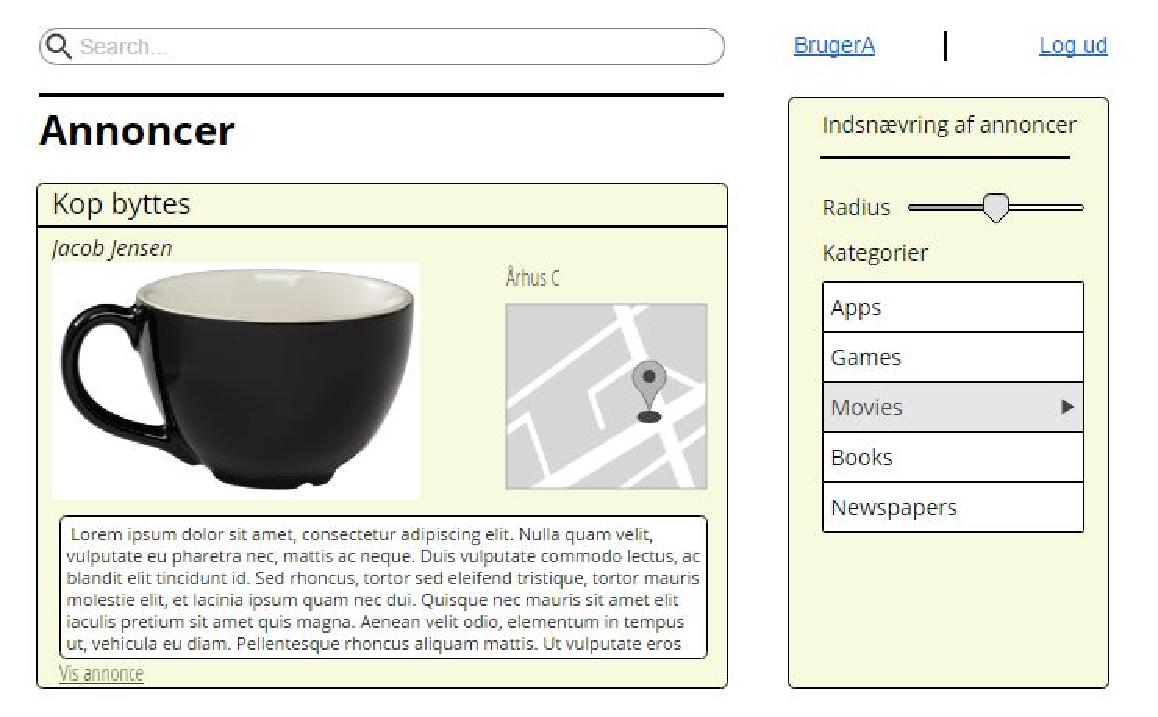
\includegraphics
	[width=165mm]
	{figures/forside.png}
	\caption{Udsnit af forsiden, hvor annoncerne vises med ejerens rating}
	\label{fig:ForsideEksempel}
\end{figure}

Når brugerne skal rate hinanden, skal de give mindst 1 stjerne. Så længe man prøver at give mindre end 1 stjerne vil det ikke være muligt at bekræfte sin rating. Denne feature er vist nedenfor på figur. Denne feature er implementeret ved hjælp af det anvendte rating plugin, som tilbyder et event, som bliver fyret når ratingens værdi ændrer sig. På den måde kan knappen ændre class mellem disabled og ikke disabled afhængig af ratingens værdi. \ref{fig:RatingEksempel}

\begin{figure}[H]
	\centering
	
\includegraphics
	[width=165mm]
	{figures/ratingconfirm.png}
	\caption{'Bekræft'-knap bliver aktiveret når man rater mindst 1 stjerne}
	\label{fig:RatingEksempel}
\end{figure}
